\chapter{Il progetto Zeri e LODE}

Come già detto in precedenza, il progetto \emph{Zeri e LODE} prevede la conversione dell'archivio della Fondazione Federico Zeri, attualmente implementato sfruttando \emph{MySQL} come RDBMS, in un corpus di triple RDF da caricare in triple store in vista dell'apertura verso la cloud LOD.

Il worflow completo di sviluppo del progetto si articola in quattro punti fondamentali (fig. \ref{fig:zerielode-steps}):
\begin{enumerate}
\item la mappatura del modello della Scheda F in CIDOC-CRM
\item la creazione del triple store
\item l'aggiunta dei collegamenti alla LOD cloud
\item la creazione dell'interfaccia di browsing
\end{enumerate}

In questa sede verranno prese in esame in particolare l'analisi e la realizzazione dei primi due punti.
\begin{figure}
    \centering
    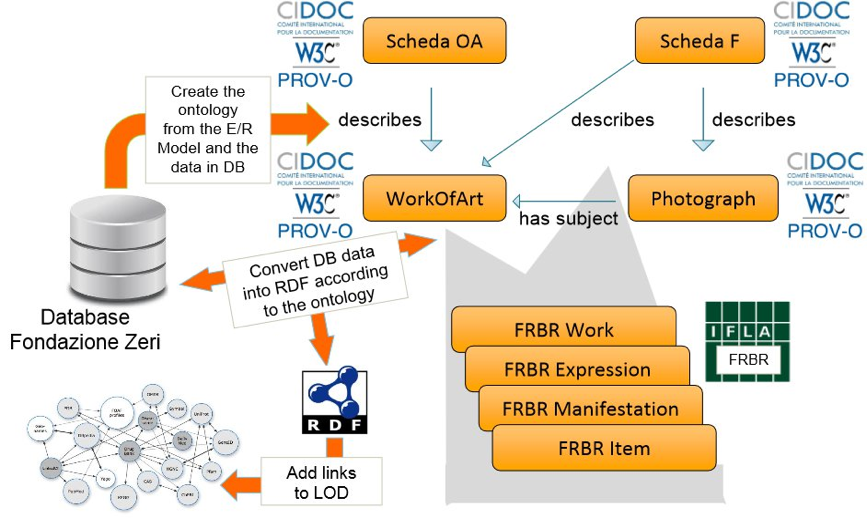
\includegraphics[width=100mm]{images/zeri-steps.png}
	\caption{Workflow di sviluppo}
	\label{fig:zerielode-steps}
\end{figure}

\section{Modello preliminare}

Per le finalità del progetto il formato ideale per l'esportazione dei dati dall'attuale archivio è stato identificato come XML (per ragioni che verranno dettagliate in~\ref{sec:data-analysis}).


\begin{figure}
    \centering
    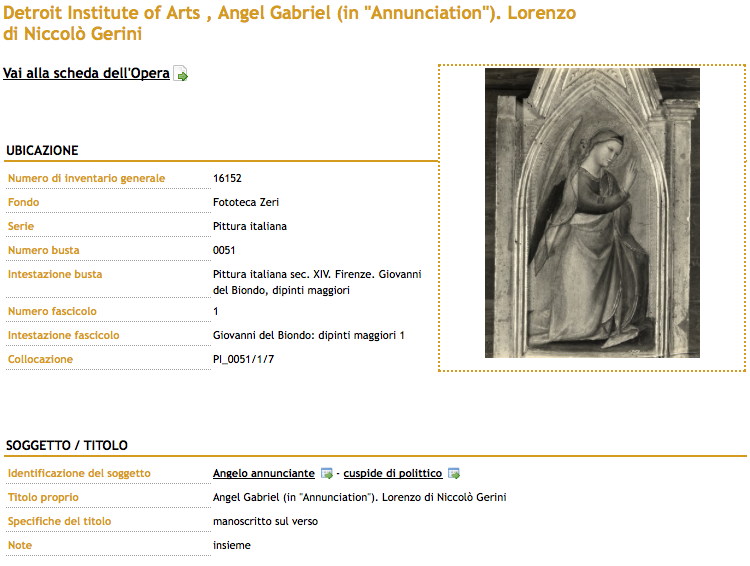
\includegraphics[width=\textwidth]{images/angelo-annunziante.png}
	\caption{Vista parziale di una scheda dell'archivio Zeri online (\protect\url{http://fe.fondazionezeri.unibo.it/catalogo/scheda.jsp?tipo_scheda=F&id=10155})}\label{fig:angelo-annunziante}
\end{figure}

\begin{noindent}
\begin{minipage}{\linewidth}
\begin{lstlisting}[caption=Esempio ideale di conversione, label=listing:conversion-example]
entryf:10155 a fentry:FEntry , crm:E31_Document ;
	crm:P1_is_identified_by "10155" ;
	crm:P70_documents photo:10155 ;
	crm:P102_has_title "Detroit Institute of Arts , Angel Gabriel (in \"Annunciation\"). Lorenzo di Niccolò Gerini." .

photo:10155 a fentry:Photograph , crm:E22_Man-Made_Object ;
	P87_is_identified_by "16152" ;
	P54_has_current_permanent_location [
		a crm:E53_Place ;
		crm:P87_is_identified_by "Giovanni del Biondo: dipinti maggiori 1" ;
		crm:P59i_is_located_on_or_within [
			a crm:E53_Place ;
			crm:P87_is_identified_by "Pittura italiana sec. XIV. Firenze. Giovanni del Biondo, dipinti maggiori" ;
			crm:P59i_is_located_on_or_within [
				a crm:E53_Place ;
				crm:P87_is_identified_by "Pittura italiana" ;
				crm:P59i_is_located_on_or_within [
					a crm:E53_Place ;
					crm:P87_is_identified_by "Fototeca Zeri" .
				] .
			] .
		] .
	] , "PI_0051/1/7" ;
	crm:P62_depicts [
		a crm:E1_CRM_Entity ;
		crm:P1_is_identified_by "Angelo annunciante - cuspide di polittico" ;
		crm:P102_has_title [
			a crm:E35_Title ;
			rdfs:label "Angel Gabriel (in \"Annunciation\"). Lorenzo di Niccolò Gerini" ;
			crm:P3_has_note "manoscritto sul verso" .
		] ;
		crm:P3_has_note "insieme" .
	] .
\end{lstlisting}
\end{minipage}
\end{noindent}

L'obiettivo finale è ottenere una conversione completa della scheda in un insieme di triple RDF. Tale conversione è stata concettualizzata, appunto, sfruttando come base le ontologie CIDOC-CRM e FRBRoo, considerando tuttavia la possibilità (e la necessità) di estenderle nel caso si fossero rivelate troppo limitate o limitanti.

Prendendo come esempio la vista parziale in fig.~\ref{fig:angelo-annunziante}, una traccia di conversione desiderata è riportata nel listato~\ref{listing:conversion-example} (un esempio completo della mappatura di un singolo record a progetto ultimato è riportata nel listato~\ref{listing:sample-output} assieme al record di partenza in XML).

Le domande informali alle quali la concettualizzazione della \emph{Scheda F} tenta di rispondere sono:
\begin{enumerate}
\item Cosa sono le Schede F e le fotografie descritte?
\item Quali sono i soggetti di tali fotografie?
\item Quali sono le entità responsabili nella descrizione degli oggetti e qual è il loro ruolo?
\item Quali sono le fotografie che rappresentano dettagli di un'opera?
\item Quali sono le fotografie in possesso di una data entità in uno specifico intervallo di tempo (e.g. la Fondazione Federico Zeri o la collezione privata dalla quale sono state acquisite)?
\item Quando sono stati creati gli oggetti e da chi?
\item Qual è la collocazione fisica delle fotografie, i.e. quali fotografie sono contenute in una specifica busta (e.g. busta 0014) e in quale fascicolo sono contenute e come sono organizzate le buste all'interno dei fascicoli?
\end{enumerate}

Durante l'analisi e lo sviluppo del progetto si è resa necessaria, per l'appunto, la creazione di un'ontologia ad hoc per poter rappresentare in modo preciso e senza perdita di specificità le varie entità coinvolte all'interno di una singola scheda. Tale ontologia è stata battezzata \emph{F Entry Ontology} (dettagliata in~\ref{sec:feo}) e sfrutta in maniera significativa altre ontologie della suite \emph{SPAR - Semantic Publishing and Referencing}\footnote{\url{http://purl.org/spar/}}.

\section{Requisiti}
Dal punto di vista tecnico la mappatura della \emph{Scheda F} doveva tener conto di diversi aspetti progettuali per poter essere un punto di riferimento, come si pone, per ulteriori sviluppi e riusi anche da parte di altre istituzioni.

Tali aspetti sono:
\begin{description}
\item[automazione] la mappatura dev'essere \emph{automatizzabile}, ovvero strutturata in modo da poter essere elaborata da una macchina quanto più possibile senza l'intervento manuale dell'uomo
\item[scalabilità] la dimensione del catalogo in input è sconosciuta, pertanto la tecnologia di conversione dev'essere pensata per sopportare cataloghi arbitrariamente grandi e pronta a scalare di conseguenza
\item[modularità] per assicurare una miglior semplicità e velocità di sviluppi futuri, la tecnologia dev'essere modulare il più possibile
\item[versatilità] offrendosi come esempio e punto di partenza per archivi diversi con diverse nature dei dati, la mappatura e la tecnologia di conversione devono essere pensate sufficientemente generiche da permettere un rapido adattamento, pur senza sacrificare la peculiarità dell'implementazione per l'archivio Zeri
\end{description}

Tali requisiti sono stati tenuti in considerazione sia nella fase di analisi e conseguente mappatura dei campi della \emph{Scheda F}, sia nel conseguente sviluppo e implementazione a livello di codice (cap.~\ref{chap:implementation})